\chapter*{Extra figures}
\addcontentsline{toc}{chapter}{Extra figures}  

\begin{figure}[ht]
    \centering
    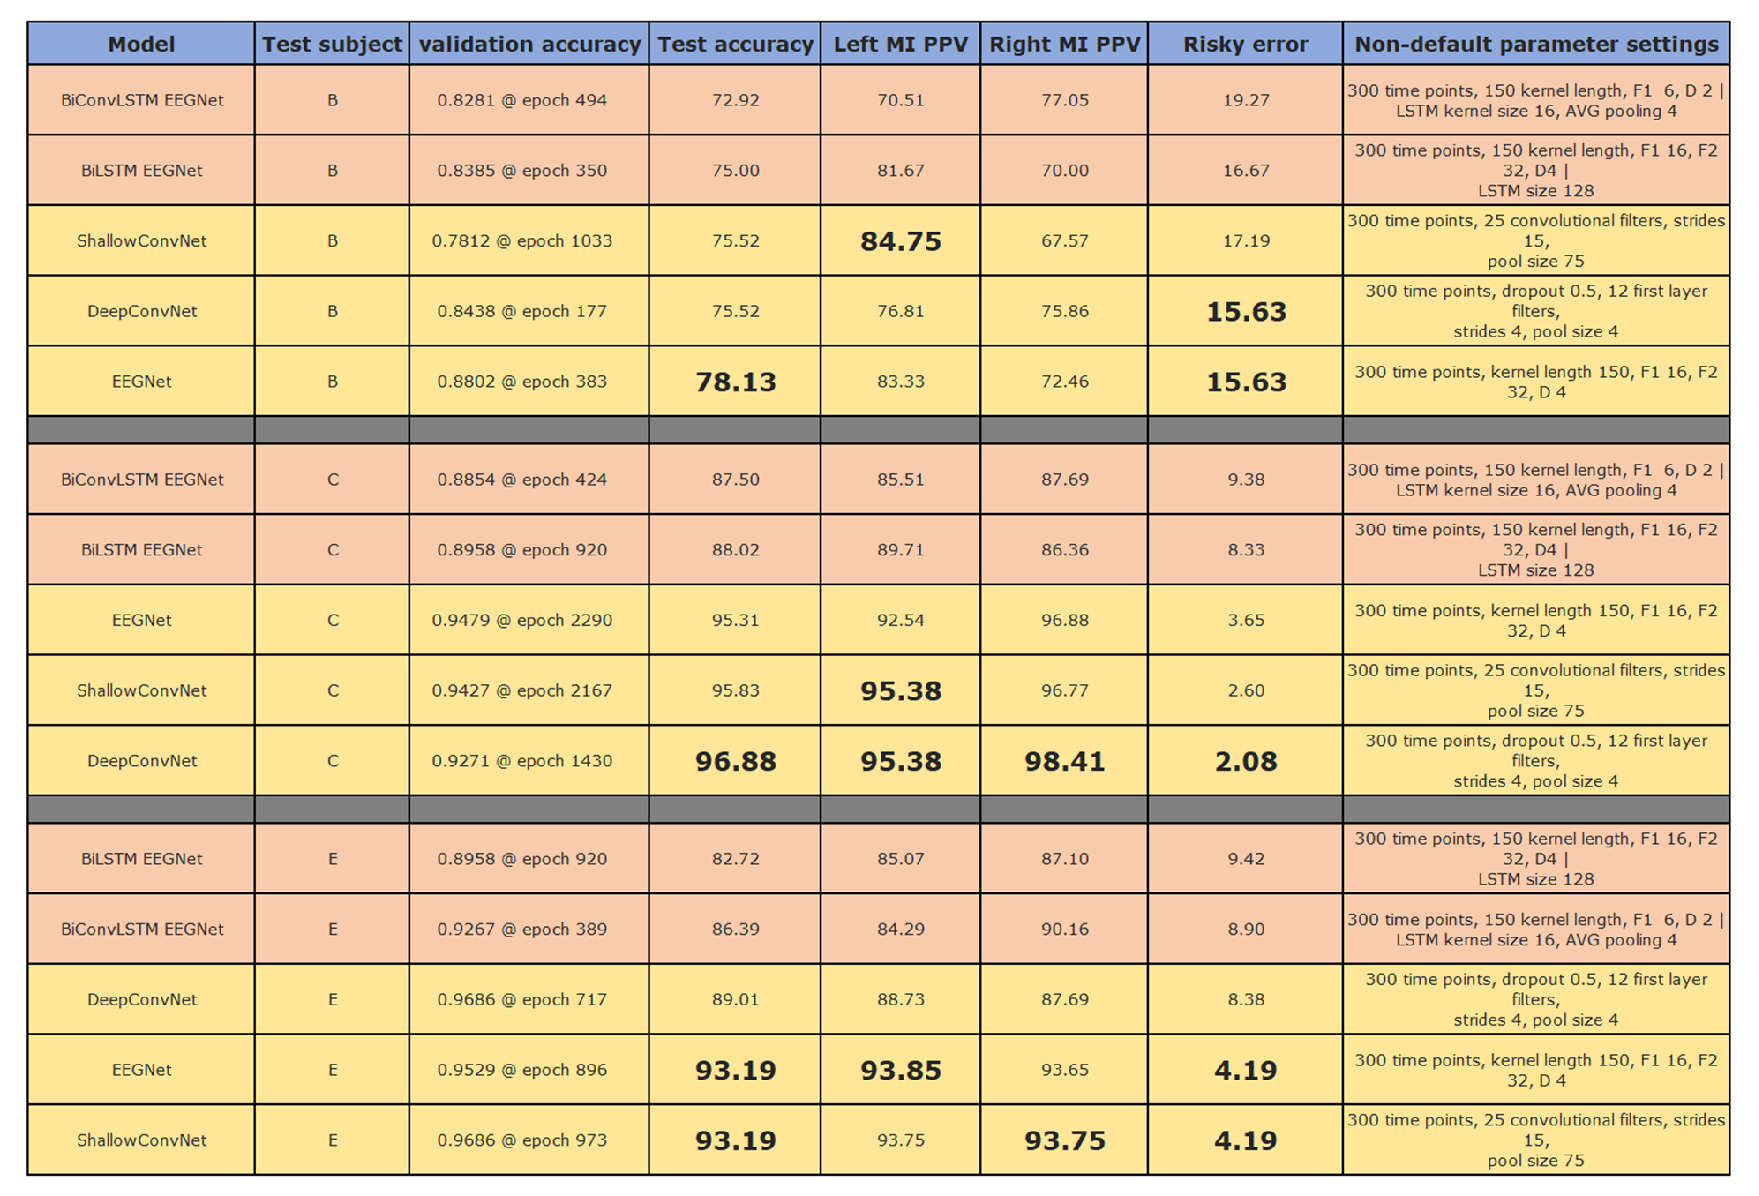
\includegraphics[width=\linewidth]{../images/results/results_intrasess_long.pdf}
    \captionsetup{width=\linewidth}
    \captionsetup{justification=centering}
    \caption{Intrasession results for all classification approaches using the longer window. Results are sorted based on the test subject and the obtained classification result on the test set. Colour codes denote either two-step \gls{csp} approaches, literature proposed \gls{cnn} approaches or master thesis proposed \gls{cnn}-\gls{lstm} approaches.} 
    \label{fig:results_intrasession_long}
\end{figure}

\begin{figure}[ht]
    \centering
    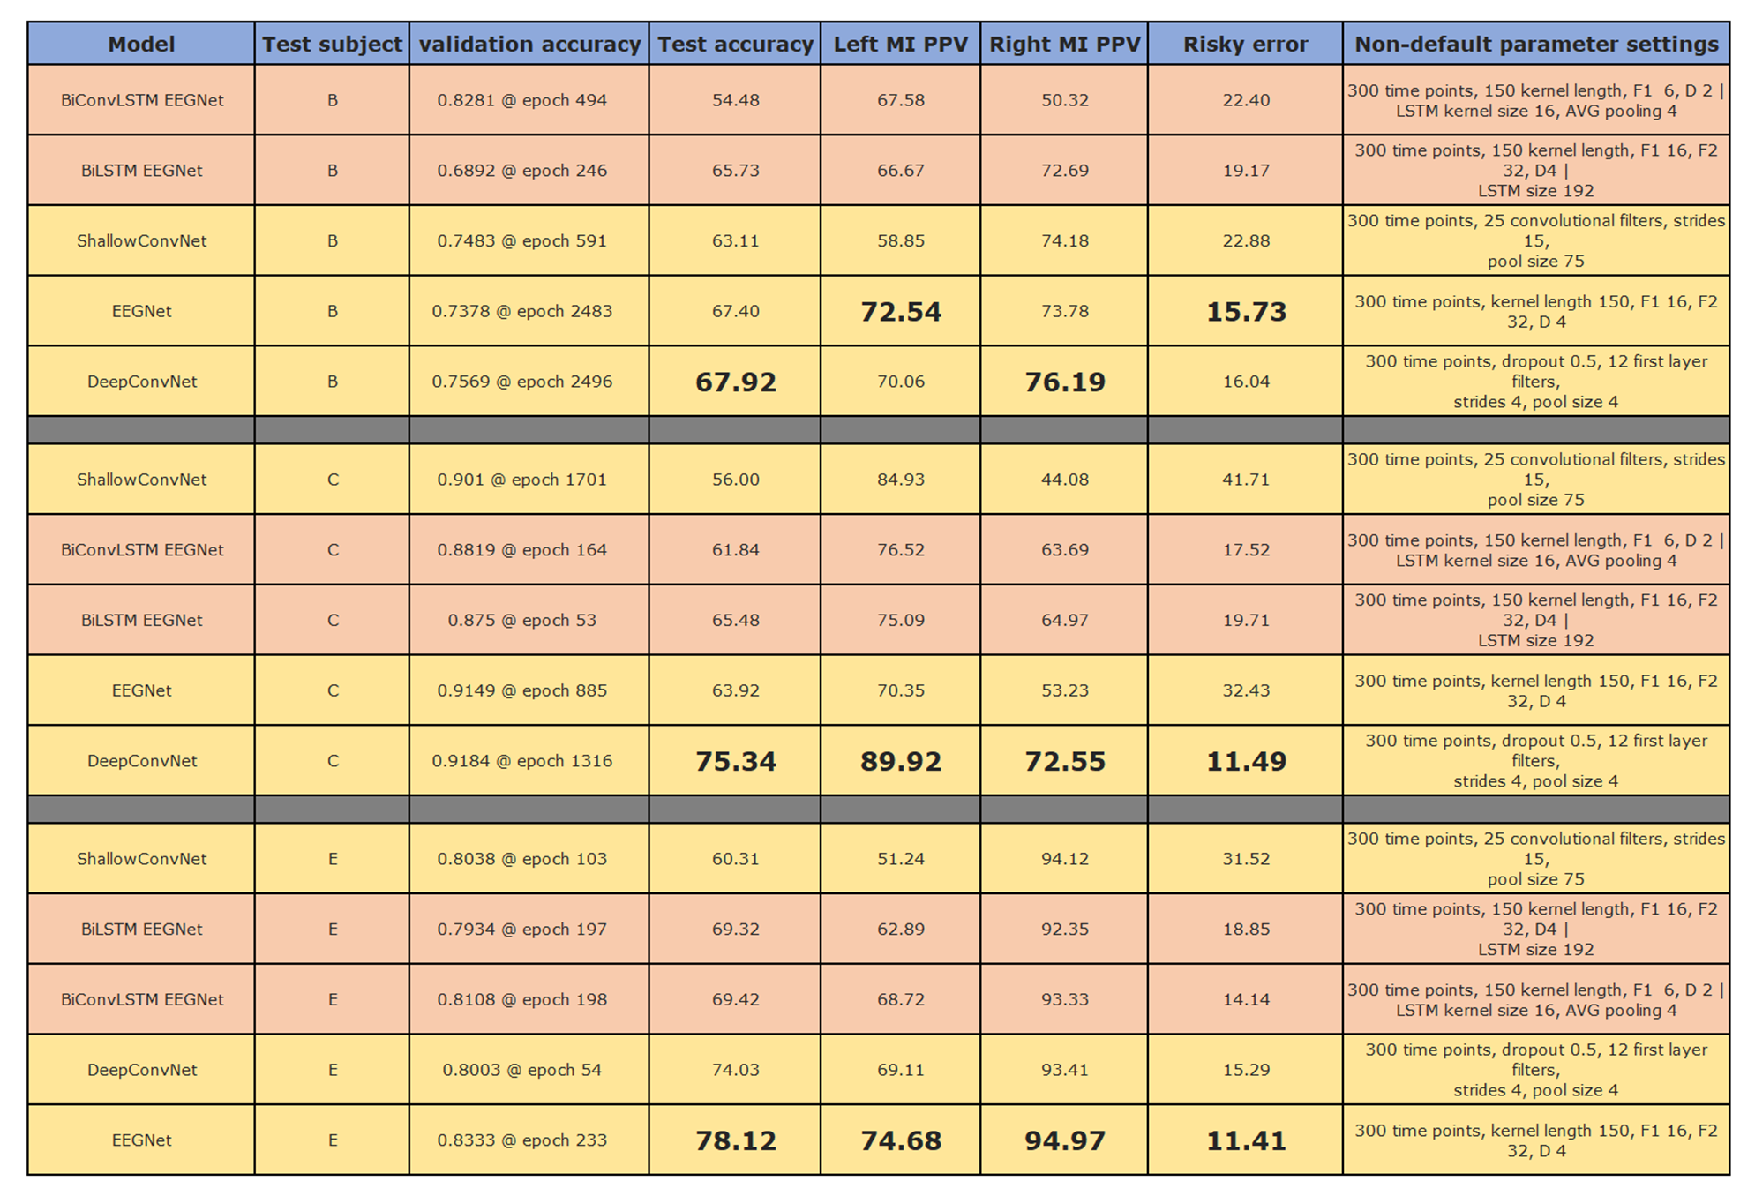
\includegraphics[width=\linewidth]{../images/results/results_intersess_long.pdf}
    \captionsetup{width=\linewidth}
    \captionsetup{justification=centering}
    \caption{Intersession results for all classification approaches using the longer window. Results are sorted based on the test subject and the obtained classification result on the test set. Colour codes denote either two-step \gls{csp} approaches, literature proposed \gls{cnn} approaches or master thesis proposed \gls{cnn}-\gls{lstm} approaches.} 
    \label{fig:results_intersession_long}
\end{figure}

\begin{figure}[ht]
    \centering
    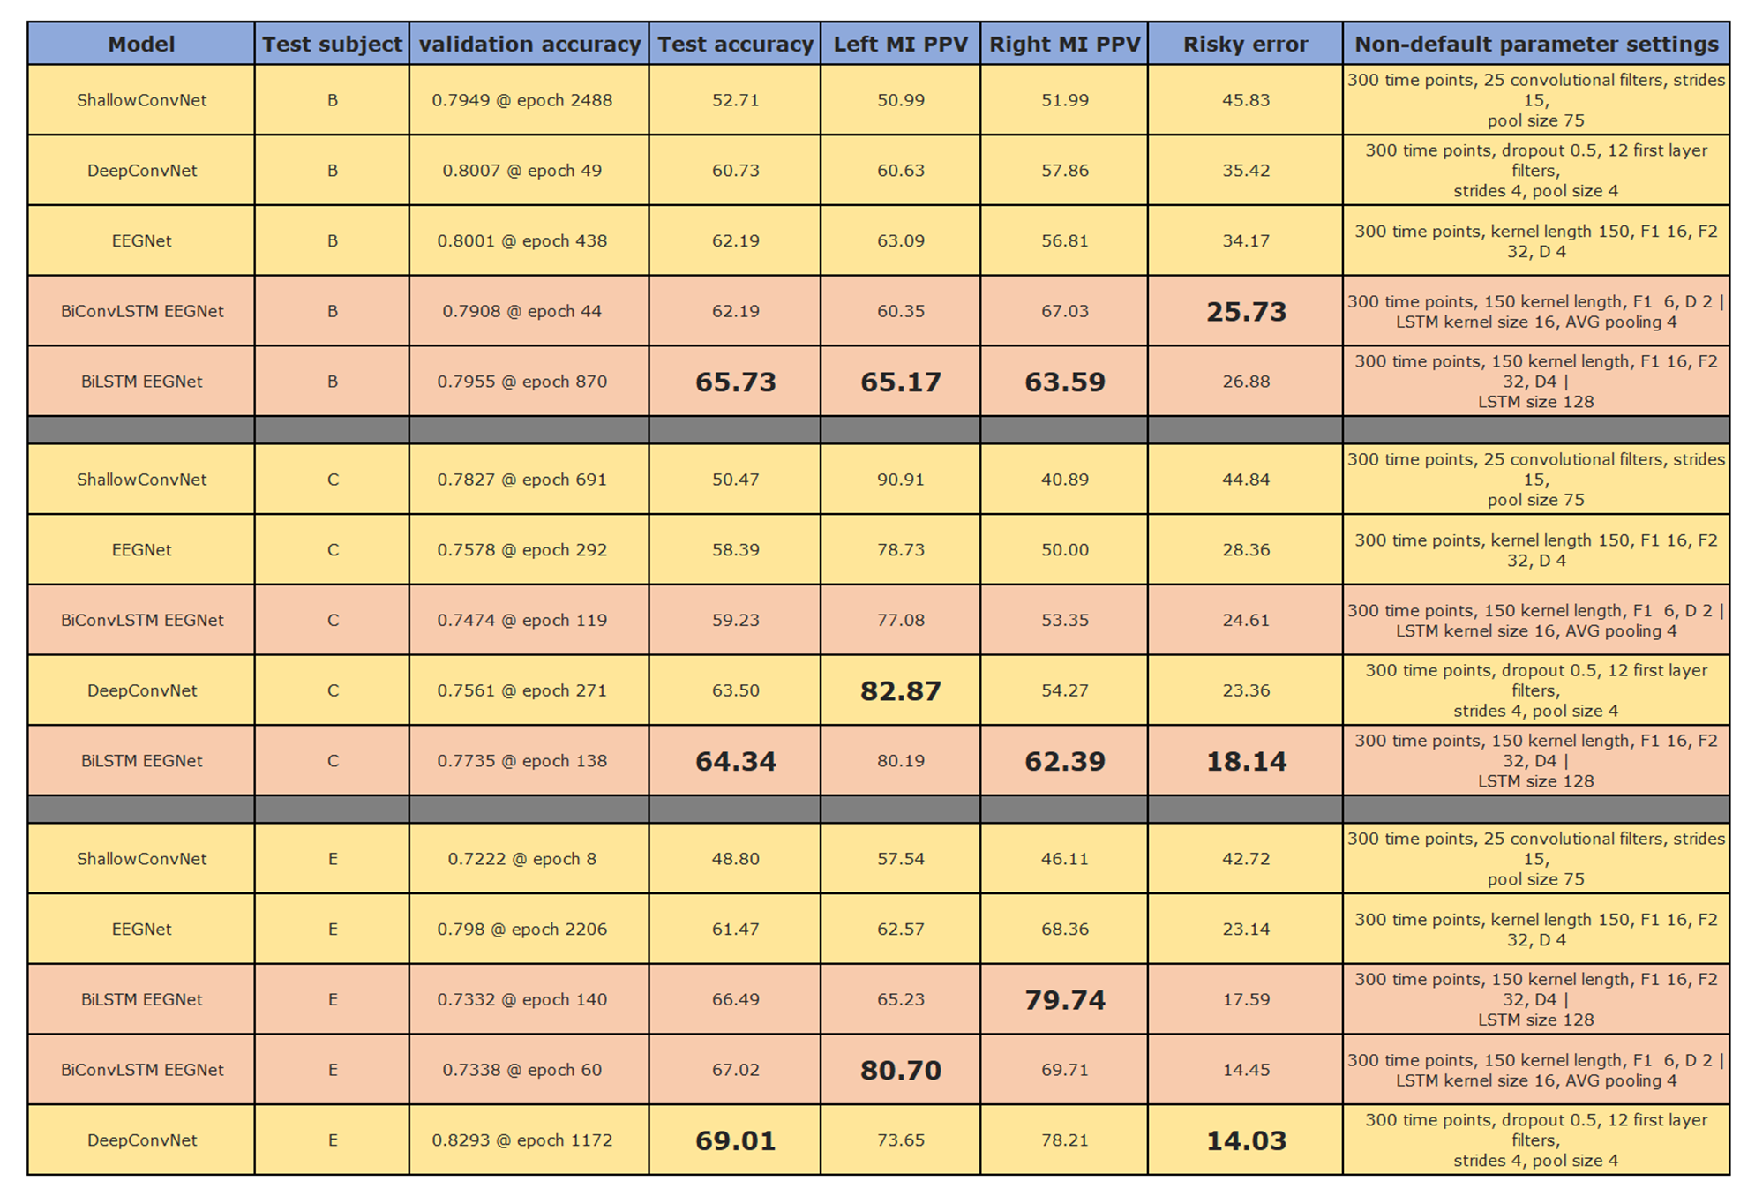
\includegraphics[width=\linewidth]{../images/results/results_intersub_long.pdf}
    \captionsetup{width=\linewidth}
    \captionsetup{justification=centering}
    \caption{Intersubject results for all classification approaches using the longer window. Results are sorted based on the test subject and the obtained classification result on the test set. Colour codes denote either two-step \gls{csp} approaches, literature proposed \gls{cnn} approaches or master thesis proposed \gls{cnn}-\gls{lstm} approaches.} 
    \label{fig:results_intersubject_long}
\end{figure}